\documentclass[8pt,xcolor=table,dvipsnames]{beamer}
\usepackage{pgfpages}
\usepackage{yhmath}
\newcommand{\Mod}[1]{\ (\mathrm{mod}\ #1)}
\providecommand{\half}{\frac{1}{2}}
\newcommand{\dg}{^\circ}
\newcommand{\arc}[1]{\wideparen{#1}}
\usetheme{Madrid}

\title{Geometric Transformations}
\subtitle{UMC K1, 2024}
\author{Nghia Doan}
\institute{MCC Club \& Competitions}
\date{\today}

\begin{document}

\section{Geometric Transformations}

\begin{frame}[t]
    \frametitle{Geometric Transformations}
    \framesubtitle{Definitions}
    A transformation is an operation that moves, flips, or changes a figure to create a new figure.

    \bigbreak
    A rigid transformation (also known as an isometry or congruence transformation)
    is a transformation that does not change the size or shape of a figure.
    
    \bigbreak
    The rigid transformations are \textit{reflections}, \textit{rotations,} and \textit{translations}.

    \begin{center}
        \includegraphics[width=4.5cm]{./svg/pdf/geo-reflection.pdf}
        \qquad
        \includegraphics[width=3.5cm]{./svg/pdf/geo-rotation.pdf}
        \qquad
        \includegraphics[width=2.5cm]{./svg/pdf/geo-translation.pdf}
    \end{center}

    The new figure created by a transformation is called the image. The original is the preimage.
\end{frame}

\section{Reflection - Example 1}

\begin{frame}[t]
    \frametitle{Geometric Transformations}
    \framesubtitle{Reflection - Example 1}
    \begin{example}
        In the right triangle $ABC$, $O$ is the midpoint of the hypotenuse $AC$.
        Points $M$ and $N$ are chosen on sides $BC$ and $BA$ such that $\angle MON = 90\dg$, $BM=4$, and $BN=3.$
        Find $AN^2 + CM^2$.
    \end{example}
    \begin{center}
        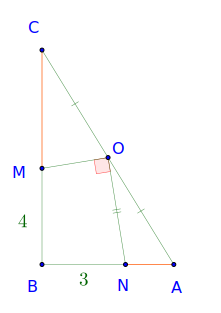
\includegraphics[width=3.9cm]{./svg/pdf/hc-2021-sm2-s2-p3-3.pdf}
    \end{center}
\end{frame}

\begin{frame}[t]
    \frametitle{Geometric Transformations}
    \framesubtitle{Reflection - Example 1 - Solution}
    \begin{center}
        \begin{overprint}
            \onslide<1>\centering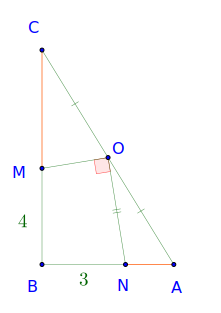
\includegraphics[width=4cm]{./svg/pdf/hc-2021-sm2-s2-p3-3.pdf}
            \onslide<2->\centering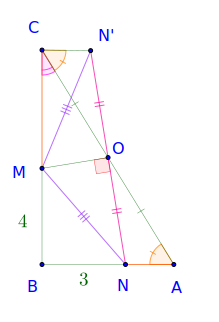
\includegraphics[width=4cm]{./svg/pdf/hc-2021-sm2-s2-p3-4.pdf}
        \end{overprint}        
    \end{center}    
    \onslide<2->{Let $N'$ be the reflection of $N$ over $O$.}
    \onslide<3->{$\triangle AON \cong \triangle CON'$ by ASA, so $AN=CN'$.}

    \onslide<4->{$\angle MCN' = \angle MCO + \angle OCN' = \angle BCA + \angle CAB = 90\dg$.
    Therefore, $\triangle ANC'$ is a right triangle.}

    \onslide<5->{$AN^2 + CM^2 = CN'^2+CN^2 = MN'^2 = MN^2 = BM^2 + BN^2 = \boxed{25.}$}
\end{frame}

\section{Reflection - Example 2}

\begin{frame}[t]
    \frametitle{Geometric Transformations}
    \framesubtitle{Reflection - Example 2}
    \begin{example}
        $\triangle ABC$ is an isosceles triangle, $AB=AC=12$, and $\angle BAC= 108\dg$. 
        Two rays $\overrightarrow{\alpha}$ and $\overrightarrow{\beta}$ starting from $A$, 
        trisect the $\angle BAC$ into three equal angles.
        Points $D$ and $E$ are the feet of the perpendiculars from $C$ and $B$ to rays $\alpha$ and $\beta$, respectively.
        Find $DE$.
    \end{example}
    \begin{center}
        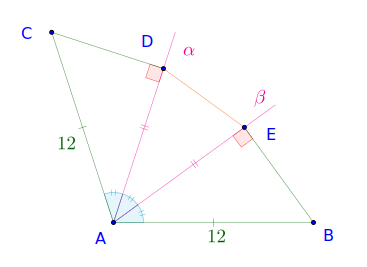
\includegraphics[width=5cm]{./svg/pdf/hc-2021-sm2-s1-p6-3.pdf}
    \end{center}
\end{frame}

\begin{frame}[t]
    \frametitle{Geometric Transformations}
    \framesubtitle{Reflection - Example 2 - Solution}
    \begin{center}
        \begin{overprint}
            \onslide<1>\centering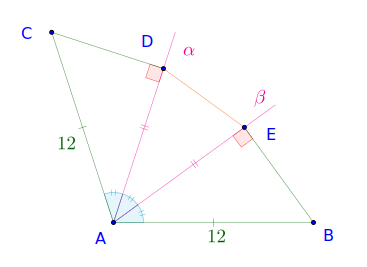
\includegraphics[width=5cm]{./svg/pdf/hc-2021-sm2-s1-p6-3.pdf}
            \onslide<2->\centering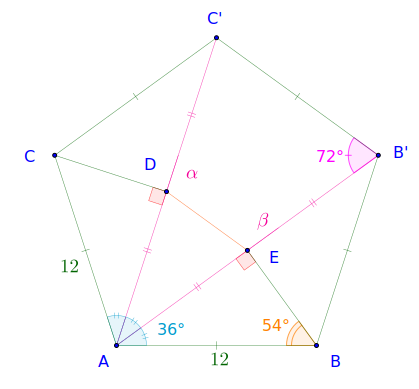
\includegraphics[width=5cm]{./svg/pdf/hc-2021-sm2-s1-p6-2.pdf}
        \end{overprint}        
    \end{center}
    \onslide<2->{Let $B'$ and $C'$ be the reflections of $A$ over lines $BE$ and $CD$, respectively.}
    
    \onslide<3->{\[ \angle B'AC + \angle CAC' = 2 \cdot 36\dg + 2 \cdot 54 \dg =  180\dg \Rightarrow CC' \parallel AB'.\]}
    \onslide<4->{Furthermore $\triangle AB'C'$ is isosceles, so $\angle B'AC = \half(180\dg - 36\dg) = 72\dg.$}

    \onslide<5->{Thus, $ACC'B'$ is isosceles trapezoid, so $B'C' = AB = 12$.}

    \onslide<6->{$DE$ is a midsegment in $\triangle AB'C'$, hence \framebox{$DE=6.$}}
\end{frame}

\section{Cyclic Quadrilaterals}

\begin{frame}[t]
    \frametitle{Geometric Transformations}
    \framesubtitle{Cyclic Quadrilaterals}
    \begin{theorem}[Cyclic Quadrilaterals]
        Let $ABCD$ be a convex quadrilateral. Then the following are equivalent:
        \begin{itemize}
            \item $ABCD$ is cyclic.
            \item $\angle ABC + \angle CDA = 180\dg$.
            \item $\angle ABD=\angle ACD$.
        \end{itemize}
    \end{theorem}
    \begin{center}
        \includegraphics[width=4cm]{./asy/pdf/cyclic-quadrilaterals-1.pdf}
        \quad
        \includegraphics[width=4cm]{./asy/pdf/cyclic-quadrilaterals-2.pdf}
    \end{center}
\end{frame}

\section{Reflection - Example 3}

\begin{frame}[t]
    \frametitle{Geometric Transformations}
    \framesubtitle{Reflection - Example 3}
    \begin{example}
        $ABCD$ is a convex quadrilateral. $BC = AD,$ $\angle DAC = 98^\circ,$ $\angle DBC = 82^\circ,$ $\angle BCD = 70^\circ.$
        Find $\angle ACD.$    
    \end{example}

    \bigbreak
    \begin{center}
        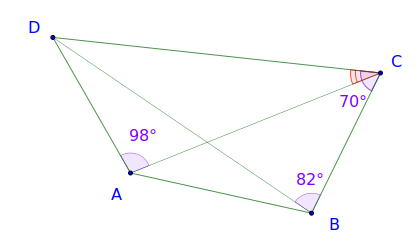
\includegraphics[width=6cm]{./svg/pdf/pct-2021-3-4-3-2-0.pdf}
    \end{center}
\end{frame}

\begin{frame}[t]
    \frametitle{Geometric Transformations}
    \framesubtitle{Reflection - Example 3 - Solution}
    \begin{center}
        \begin{overprint}
            \onslide<1>\centering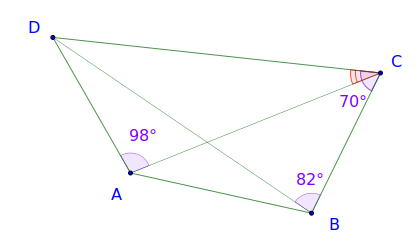
\includegraphics[width=6cm]{./svg/pdf/pct-2021-3-4-3-2-0.pdf}
            \onslide<2->\centering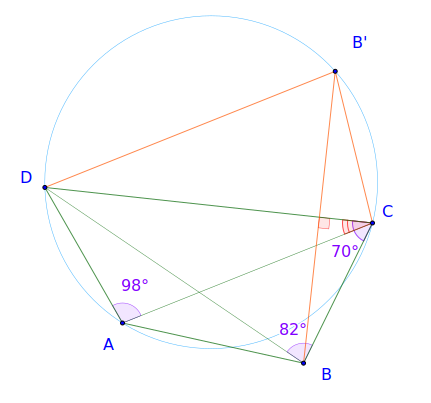
\includegraphics[width=6cm]{./svg/pdf/pct-2021-3-4-3-2-1.pdf}
        \end{overprint}        
    \end{center}
    \onslide<2->{Let $B'$ be the reflection of $B$ across $CD$.}
    \onslide<3->{$\angle DAC+\angle CB'D=180^\circ,$ so $ACB'D$ is cyclic. $AD=BC,$ thus $\arc{AD} = \arc{BC}.$}
    \onslide<4->{Therefore $\angle ACB'= \angle DAC = 98^\circ$.}
    \onslide<5->{\[
        \angle DCB'=\angle BCD=70^\circ \Rightarrow \angle ACD=\angle ACB'-\angle DCB'=98^\circ-70^\circ=\boxed{28^\circ.}
    \]}
\end{frame}

\section{Reflection - Example 4}

\begin{frame}[t]
    \frametitle{Geometric Transformations}
    \framesubtitle{Reflection - Example 4}
    \begin{example}
        Let $G$ be the centroid of $\triangle ABC.$ If $\angle AGB \le 90\dg,$
        find the largest possible value of $n$ integer, such that $AC + CB > n AB.$
    \end{example}

    \bigbreak
    \begin{center}
        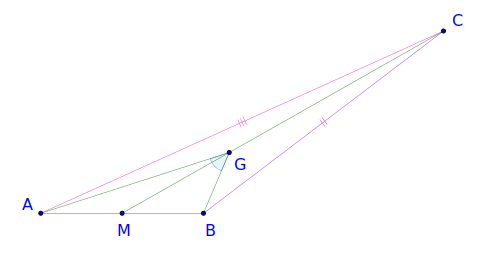
\includegraphics[width=8cm]{./svg/pdf/pct-2021-3-5-4-2-0.pdf}
    \end{center}
\end{frame}

\begin{frame}[t]
    \frametitle{Geometric Transformations}
    \framesubtitle{Reflection - Example 4 - Solution}
    \begin{center}
        \begin{overprint}
            \onslide<1>\centering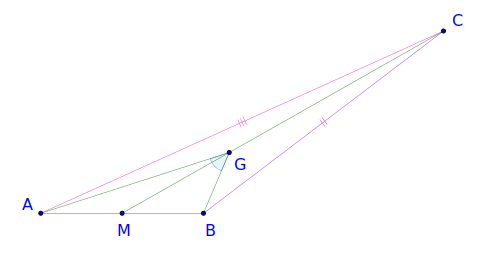
\includegraphics[width=8cm]{./svg/pdf/pct-2021-3-5-4-2-0.pdf}
            \onslide<2->\centering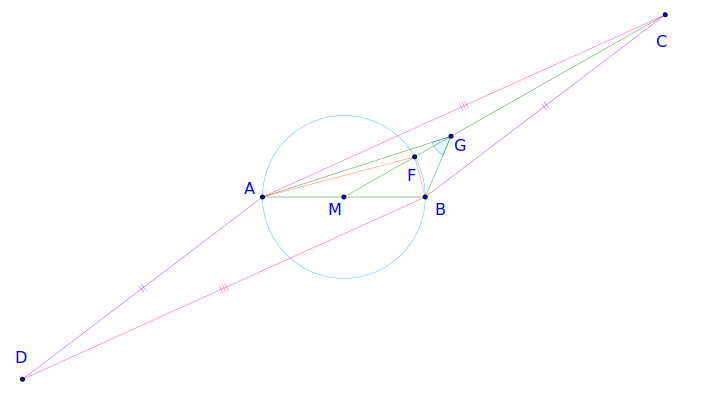
\includegraphics[width=9cm]{./svg/pdf/pct-2021-3-5-4-2-1.pdf}
        \end{overprint}        
    \end{center}
    \onslide<2->{Let $M$ be the midpoint of $AB,$ $F$ be the intersection of the circle centred $M$ diameter $AB.$ 
    $AGB \le 90\dg$ so $G$ is outside the circle $(M)$, therefore $GM \le FM= \half AB.$}

    \onslide<3->{Let $D$ be the reflection of $C$ over $M$. In triangle $DAC$, $DA+AC>DC \Rightarrow AB+AC>2CM.$}
    
    \onslide<4->{Therefore $AB \le 2 GM = \frac{2}{3} CM < \frac{1}{3} (AB+AC),$ thus $AB+AC>3AB.$}

    \onslide<5->{If $AC = BC,$ $G$ on circle $(M)$, then $AB+AC=\sqrt{10}AB<4AB.$ Thus, \framebox{$n=3.$}}
\end{frame}

\section{Reflection - Example 5}

\begin{frame}[t]
    \frametitle{Geometric Transformations}
    \framesubtitle{Reflection - Example 5}
    \begin{example}
        $A, B$ are two points on the circle. A curve through $A, B$ bisects the area of the circle.
        Prove that the curve is at least as long as a diameter of the circle.    
    \end{example}

    \bigbreak
    \begin{center}
        \includegraphics[width=5cm]{./svg/pdf/23-24-sm2-s3-ci-p10.pdf}
    \end{center}
\end{frame}

\begin{frame}[t]
    \frametitle{Geometric Transformations}
    \framesubtitle{Reflection - Example 5 - Solution}
    \begin{center}
        \begin{overprint}
            \onslide<1>\centering\includegraphics[width=5cm]{./svg/pdf/23-24-sm2-s3-ci-p10.pdf}
            \onslide<2->\centering\includegraphics[width=5cm]{./svg/pdf/23-24-sm2-s3-ci-p10-1.pdf}
        \end{overprint}        
    \end{center}
    It is obvious that the curve is at least as long as a diameter of the circle if $AB$ is a diameter.
    Thus, let's assume that $AB$ is a chord that is shorter than the diameter of the circle.

    \onslide<2->{Let $CD$ be the diameter of the circle that is parallel to $AB.$ Let $B'$ be the reflection of $B$ over $CD.$}

    \onslide<3->{If the curve does not intersect $CD,$ then the curve cannot bisect the area of the circle, thus the curve must intersect $CD.$}
    
    \onslide<4->{Let one of the intersections be $E$. The length of the curve must be at least as long as $BE + EA.$
    Now, $BE + EA = B'E + EA \ge B'A,$ which is a diameter.}

    \onslide<5->{Hence, the curve is at least as long as a diameter of the circle.}
\end{frame}

\section{Reflection - Example 6}

\begin{frame}[t]
    \frametitle{Geometric Transformations}
    \framesubtitle{Reflection - Example 6}
    \begin{example}
        A continuous curve split an unit equilateral triangle $ABC$ into two regions with equal area.
        What is the minimal length of the curve?    
    \end{example}

    \bigbreak
    \begin{center}
        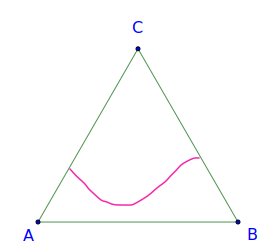
\includegraphics[width=4.5cm]{./svg/pdf/24-25-t4-p20.pdf}
    \end{center}
\end{frame}

\begin{frame}[t]
    \frametitle{Geometric Transformations}
    \framesubtitle{Reflection - Example 6 - Solution}
    \begin{center}
        \begin{overprint}
            \onslide<1>\centering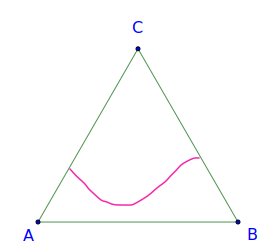
\includegraphics[width=4.5cm]{./svg/pdf/24-25-t4-p20.pdf}
            \onslide<2->\centering\includegraphics[width=6cm]{./svg/pdf/24-25-t4-p20-2.pdf}
        \end{overprint}        
    \end{center}
    \onslide<2->{The continuous curve becomes a close curve encompassing an area half of a unit circle, or $\pi.$}

    \onslide<3->{The close curve encompassing an area has minimal length if it forms the perimeter of a circle.}
    
    \onslide<4->{This circle has an area of $\half \pi,$ thus its radius of $\frac{1}{\sqrt{2}}$
    and a perimeter of $2\pi \left( \frac{1}{\sqrt{2}} \right) = \pi\sqrt{2}.$}

    \onslide<5->{Therefore the minimal length of the original curve is one-sixth of $\pi\sqrt{2},$ which is $\frac{\pi \sqrt{2}}{6}.$}
\end{frame}

\section{Reflection - Example 7}

\begin{frame}[t]
    \frametitle{Geometric Transformations}
    \framesubtitle{Reflection - Example 7}
    \begin{example}
        A circle has center on the side $AB$ of the cyclic quadrilateral $ABCD$.
        The other three sides are tangent to the circle. Prove that $AD + BC = AB$.    
    \end{example}

    \bigbreak
    \begin{center}
        \includegraphics[width=4.5cm]{./svg/pdf/imo-1985-1-1.pdf}
    \end{center}
\end{frame}

\begin{frame}[t]
    \frametitle{Geometric Transformations}
    \framesubtitle{Reflection - Example 7 - Solution}
    \begin{center}
        \begin{overprint}
            \onslide<1>\centering\includegraphics[width=4.5cm]{./svg/pdf/imo-1985-1-1.pdf}
            \onslide<2->\centering\includegraphics[width=4.5cm]{./svg/pdf/imo-1985-1-4.pdf}
        \end{overprint}        
    \end{center}
    \onslide<2->{Let $E$ be the intersection of $AD$ and $BC$. Let $A'$ and $B'$ be the reflections of $A$ and $B$ over $EO.$}

    \onslide<3->{\[ \angle EA'B' = \angle EAB = \angle ECD \Rightarrow CD \parallel A'B' \Rightarrow \angle DCO = \angle COA'. \]}
    \onslide<4->{$CB, CD$ are tangents, so $CO$ is the bisector of $\angle DCB,$ therefore \[ \angle DCO = \angle OCA' \Rightarrow \angle COA' = \angle OCA'. \]}
    \onslide<5->{Thus, $OA'=CA',$ so $OA=OA'=CA'=DA,$ similarly $OB=CB.$}
    \onslide<6->{Hence, \framebox{$AD + BC = AB.$}}
\end{frame}

\section{Ptolemy Inequality}

\begin{frame}[t]
    \frametitle{Geometric Transformations}
    \framesubtitle{Ptolemy Inequality}
    \begin{theorem}[Ptolemy Inequality]
        \label{theorem:ptolemy-inequality}
        The inequality states that in for four points $A, B, C, D$ in the plane,
        \[
            AB \cdot CD + BC \cdot DA \ge AC \cdot BD,
        \]
        with equality for any \textit{cyclic quadrilateral} $ABCD$ with diagonals $AC$ and $BD$.
    \end{theorem}
    \begin{center}
        \includegraphics[width=4.5cm]{./svg/pdf/ptolemy-inequality-1.pdf}
    \end{center}
    \textit{Note: this also holds if $A,B,C,D$ are four points not in the same plane, but the equality can't be achieved.}
\end{frame}

\begin{frame}[t]
    \frametitle{Geometric Transformations}
    \framesubtitle{Ptolemy Inequality - Proof}
    \begin{center}
        \includegraphics[width=4.5cm]{./svg/pdf/ptolemy-inequality-1.pdf}
    \end{center}
    \begin{proof}
        \onslide<2->{Let $E$ be the point such that $\angle EAB=\angle CDB,\ \angle EBA=\angle CBD.$}
        \onslide<3->{\[ \triangle AEB \sim \triangle DCB \Rightarrow \triangle ADB \sim \triangle CEB 
        \Rightarrow \frac{AE}{CD} = \frac{AB}{BD},\ \frac{CE}{AD}=\frac{BC}{BD}. \]}
        \onslide<4->{\[ AE+CE \ge AC \Rightarrow AE+CE=\frac{AB \cdot CD + BC \cdot AD}{BD} \ge AC
        \Rightarrow AB \cdot CD + BC \cdot AD \ge AC \cdot BD.\]}
        \onslide<6->{The equality stands if and only if $E \in AC,$ or $\angle CAB=\angle EAB=\angle CDB$, so $ABCD$ is cyclic.}
    \end{proof}
\end{frame}

\section{Pompeiu's Theorem}

\begin{frame}[t]
    \frametitle{Geometric Transformations}
    \framesubtitle{Pompeiu's Theorem}
    \begin{theorem}[Pompeiu's Theorem]
        \label{theorem:pompeiu-theorem}
        $\triangle ABC$ is equilateral.
        For any point $M$, the segments $AM$, $BM$ and $CM$ form a triangle.
        This triangle degenerates if and only if $M$ lies on the circumcircle of $\triangle ABC$.
    \end{theorem}
    
    \bigbreak
    \begin{center}
        \includegraphics[width=5cm]{./svg/pdf/pompeiu-theorem-1.pdf}
    \end{center}
\end{frame}

\begin{frame}[t]
    \frametitle{Geometric Transformations}
    \framesubtitle{Pompeiu's Theorem - Proof}
    \begin{center}
        \includegraphics[width=5cm]{./svg/pdf/pompeiu-theorem-1.pdf}
    \end{center}
    \begin{proof}
        \onslide<2->{If $M$ is inside of $\triangle ABC$, then $AM+BM > AB > CM$.}
        \onslide<3->{If $M$ is outside of $\triangle ABC$, by \nameref{theorem:ptolemy-inequality}, for four points $A,B,C,M$
        \[ AM \cdot BC + CM \cdot AB \ge BC \cdot BM \Rightarrow AM + CM \ge BM. \]}
        \onslide<4->{Similarly with other triangle inequalities. Hence, \framebox{$AM$, $BM$ and $CM$ form a triangle.}}

        \onslide<5->{The equality stands if and only if $ABCM$ is cyclic, or $M$ is on the circumcircle of $\triangle ABC$.}
    \end{proof}
\end{frame}

\section{Reflection - Example 8}

\begin{frame}[t]
    \frametitle{Geometric Transformations}
    \framesubtitle{Reflection - Example 8}
    \begin{example}
        Let $ABCDEF$ be a convex hexagon with $AB = BC = CD$ and $DE = EF = FA$,
        such that $\angle BCD = \angle EFA = \frac {\pi}{3}$.
        Suppose $G$ and $H$ are points in the interior of the hexagon
        such that $\angle AGB = \angle DHE = \frac {2\pi}{3}$.
        Prove that $AG + GB + GH + DH + HE \geq CF$.
    \end{example}

    \bigbreak
    \begin{center}
        \includegraphics[width=6cm]{./svg/pdf/imo-1995-5-1.pdf}
    \end{center}
\end{frame}

\begin{frame}[t]
    \frametitle{Geometric Transformations}
    \framesubtitle{Example 8 - Solution}
    \begin{center}
        \begin{overprint}
            \onslide<1>\centering\includegraphics[width=6cm]{./svg/pdf/imo-1995-5-1.pdf}
            \onslide<2->\centering\includegraphics[width=6cm]{./svg/pdf/imo-1995-5-2.pdf}
        \end{overprint}
    \end{center}
    \begin{overprint}
        \onslide<2>$\triangle BCD, \triangle EFA$ are equilateral, so $AE=ED, DB=BA$, thus $BE$ is an axis of symmetry of $ABDE.$
        Let $C'$ and $F'$ be the reflections of $C$ and $F$ over the line $BE$, respectively.
        \onslide<3>$\triangle AC'B$ is the reflection of $\triangle DBC$, hence $\angle AC'B = \angle BCD = 60\dg.$
        $\angle AGB = 120\dg$, so $G$, by the property of cyclic-quadrilaterals, lies on the circle $(ABC').$
        \onslide<4>Similarly $H$ lies on the circle $(DEF').$
        \onslide<5>Thus, according to by Pompeiu's Theorem, $AG+GB=C'G$ and $DH+HE=HF'$, so
        \[ AG + GB + GH + DH + HE = C'G + GH + HF' \ge C'F'= CF \]
        \onslide<6>Hence, \framebox{$AG + GB + GH + DH + HE \geq CF$.}
    \end{overprint}
\end{frame}

\section{Menelaus Theorem}

\begin{frame}[t]
    \frametitle{Geometric Transformations}
    \framesubtitle{Menelaus Theorem}
    \begin{theorem}[Ceva Theorem]
        Let $ABC$ be a triangle, and let $D, E, F$ be points on lines $BC, CA, AB$, respectively.
        Lines $AD, BE, CF$ are \textcolor{orange}{concurrent} \textit{if and only if}:
        $\dfrac{BD}{DC} \cdot \dfrac{CE}{EA}\cdot \dfrac{AF}{FB} = 1.$
    \end{theorem}
    \begin{center}
        \includegraphics[width=7.5cm]{./svg/pdf/ceva-menelaus.pdf}
    \end{center}
    \begin{theorem}[Menelaus Theorem]
        Let $ABC$ be a triangle, and let $D,F$ be points on lines $BC,AB$, respectively.
        $E$ is on the extension of $CA$.
        Points $D, E, F$ are \textcolor{orange}{collinear} \textit{if and only if}:
        $\dfrac{BD}{DC} \cdot \dfrac{CE}{EA}\cdot \dfrac{AF}{FB} = 1.$
    \end{theorem}
\end{frame}

\section{Rotation - Example 1}

\begin{frame}[t]
    \frametitle{Geometric Transformations}
    \framesubtitle{Rotation - Example 1}
    \begin{example}
        Point $B$ lies on a line which is tangent to circle $\omega$ at point $A.$
        The line segment $AB$ is rotated about the center of the circle by some angle to form segment $A'B'.$
        prove that the line $AA'$ bisects the segment $BB'.$
    \end{example}

    \bigbreak
    \begin{center}
        \includegraphics[width=5cm]{./svg/pdf/sc-23-hs-3-p7.pdf}
    \end{center}
\end{frame}

\begin{frame}[t]
    \frametitle{Geometric Transformations}
    \framesubtitle{Rotation - Example 1 - Solution}
    \begin{center}
        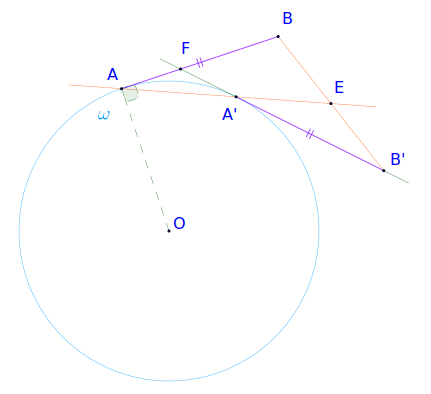
\includegraphics[width=5cm]{./svg/pdf/sc-23-hs-3-p7-2.pdf}
    \end{center}
    \onslide<2->{Let $E$ be the intersections of lines through $AA'$ and $BB'.$ 
    Let $F$ be the intersections of lines through $AB$ and $A'B'.$}
    \onslide<3->{$FA$ and $FA'$ are both tangents of $\omega,$ so $FA = FA'.$
    $A'B'$ is the image of the rotation of $AB$ about the center of $\omega,$ thus $A'B' = AB.$}
    \onslide<4->{By Menelaus Theorem, for $\triangle B'BF$:
    \[
        \frac{B'E}{EB} \cdot \frac{BA}{AF} \cdot \frac{FA'}{A'B'} = 1 \Rightarrow \frac{B'E}{EB} = 1 \Rightarrow 
        \boxed{AA' \text{\ bisects\ } BB'}.
    \]}
\end{frame}

\section{Rotation - Example 2}

\begin{frame}[t]
    \frametitle{Geometric Transformations}
    \framesubtitle{Rotation - Example 2}
    \begin{example}
        Given isosceles triangle $ABC,$ $AB = BC,$ and $\angle B = 20\dg,$ prove that $AB < 3AC.$
    \end{example}

    \bigbreak
    \begin{center}
        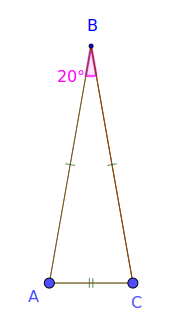
\includegraphics[width=3cm]{./svg/pdf/24-25-t4-p8-0.pdf}
    \end{center}
\end{frame}

\begin{frame}[t]
    \frametitle{Geometric Transformations}
    \framesubtitle{Rotation - Example 2 - Solution}
    \begin{center}
        \begin{overprint}
            \onslide<1>\centering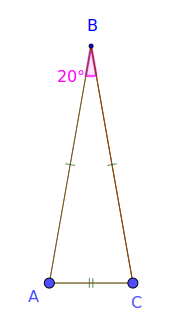
\includegraphics[width=3cm]{./svg/pdf/24-25-t4-p8-0.pdf}
            \onslide<2->\centering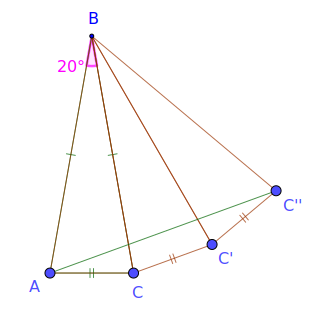
\includegraphics[width=5cm]{./svg/pdf/24-25-t4-p8.pdf}
        \end{overprint}        
    \end{center}
    \onslide<2->{Let's rotate the triangle $ABC$ around $B$ twice $20\dg$ as shown in the diagram above.}

    \onslide<3->{Then $ABE$ is a equilateral triangle, $AB = AC'' < AC + CC' + C'C'' = 3AC.$}
\end{frame}

\section{Rotation - Example 3}

\begin{frame}[t]
    \frametitle{Geometric Transformations}
    \framesubtitle{Rotation - Example 3}
    \begin{example}
        Given a triangle $ABC$ with $AB>BC$, let $\omega $ be the circumcircle.
        Let $M$, $N$ lie on the sides $AB$, $BC$ respectively, such that $AM=CN$.
        Let $K$ be the intersection of $MN$ and $AC$.
        Let $P$ be the incentre of the triangle $AMK$ and $Q$ be the $K$-excentre of the triangle $CNK$.
        If $R$ is midpoint of the arc $ABC$ of $\omega $ then prove that $RP=RQ$.
    \end{example}

    \bigbreak
    \begin{center}
        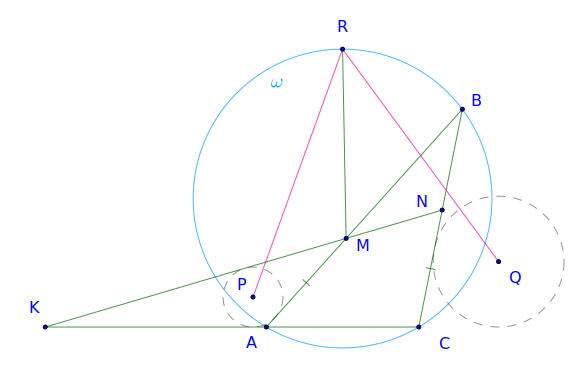
\includegraphics[width=7cm]{./svg/pdf/24-25-t3-p15-0.pdf}
    \end{center}
\end{frame}

\begin{frame}[t]
    \frametitle{Geometric Transformations}
    \framesubtitle{Rotation - Example 3 - Solution}
    \begin{center}
        \begin{overprint}
            \onslide<1>\centering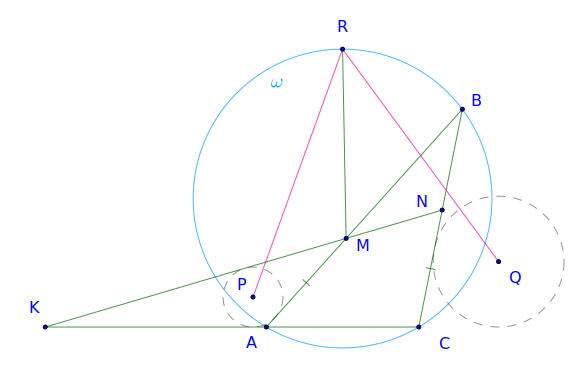
\includegraphics[width=7cm]{./svg/pdf/24-25-t3-p15-0.pdf}
            \onslide<2->\centering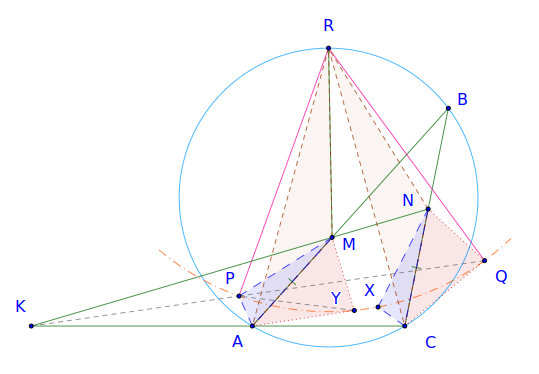
\includegraphics[width=7cm]{./svg/pdf/24-25-t3-p15.pdf}
        \end{overprint}        
    \end{center}
    \begin{overprint}
        \onslide<2>Note that $\triangle RMA \cong \triangle RNC,$ hence $R$ is the rotation center of $\overline{AM} \mapsto \overline{CN}$.
        Rotate about $R$ such that $\triangle CNQ \mapsto \triangle AMY$ and $\triangle AMP \mapsto \triangle CNX$.
        We prove that $P,Q,X,Y$ are concyclic.
        \onslide<3>First, $\angle APM+\angle CQN=180^{\circ},$ so $APMY$ and $CXNQ$ are congruent cyclic quadrilaterals.
        Since $K, P, Q$ are colinear:
        \[
            \begin{aligned}
                &\angle APQ = 180\dg - \angle KPA = \angle PKA + \angle PAK = \tfrac{1}{2}\left(\angle KAM+\angle MKA\right)
                = 90\dg - \tfrac{1}{2} \angle BMN\\
                &\angle YPQ = \angle APQ-\angle APY=  (90^{\circ}-\tfrac{1}{2} \angle BMN) - \tfrac{1}{2}\angle BNM
                =\tfrac{1}{2}\angle ABC. 
            \end{aligned}
        \]
        \onslide<4>Similarly, we get $\angle XQP=\tfrac{1}{2}\angle ABC$. Thus $\angle YPQ=\angle XQP.$
        Since $YP=XQ$, $PQXY$ is an isosceles trapezoid.
        Therefore $RP=RX$ and $RQ=RY$, we conclude that $R$ is the center of the circle $\odot(PQXY)$.
        Hence $RP=RQ$, as desired.
    \end{overprint}        
\end{frame}

\section{Translation - Example 1}

\begin{frame}[t]
    \frametitle{Geometric Transformations}
    \framesubtitle{Translation - Example 1}
    \begin{example}
        The point $O$ is situated inside the parallelogram $ABCD$ such that $\angle AOB+\angle COD=180^{\circ}$.
        Prove that $\angle OBC=\angle ODC$.
    \end{example}

    \bigbreak
    \begin{center}
        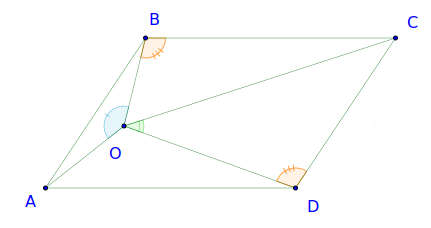
\includegraphics[width=8cm]{./svg/pdf/canada-mo-1997-4-0.pdf}
    \end{center}
\end{frame}

\begin{frame}[t]
    \frametitle{Geometric Transformations}
    \framesubtitle{Translation - Example 1 - Solution}
    \begin{center}
        \begin{overprint}
            \onslide<1>\centering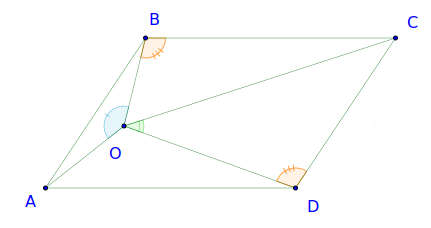
\includegraphics[width=8cm]{./svg/pdf/canada-mo-1997-4-0.pdf}
            \onslide<2->\centering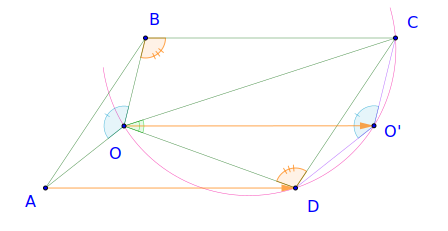
\includegraphics[width=8cm]{./svg/pdf/canada-mo-1997-4-1.pdf}
        \end{overprint}        
    \end{center}
    \onslide<2->{The translation by $\overrightarrow{AD}$ maps $A$ to $D$, $B$ to $C$, and $O$ to $O'$.}

    \bigbreak
    \onslide<3->{$ABCD$ is a parallelogram, $AD \parallel BC, AD = BC.$
    By the translation, $OO' \parallel AD, OO' = AD,$ thus $OO' \parallel BC, OO' = BC.$ 
    Therefore $OBCO'$ is a parallelogram. It implies that $\angle OBC = \angle OO'C.$}

    \bigbreak
    \onslide<4->{Since $\angle AOB+\angle COD=180^{\circ}$, so $\angle DO'C + \angle COD = 180\dg,$ or $CODO'$ is cyclic.
    Therefore $\angle ODC = \angle OO'C.$ Hence, $\boxed{\angle OBC = \angle ODC.}$}
\end{frame}

\section{Homothety}

\begin{frame}[t]
    \frametitle{Geometric Transformations}
    \framesubtitle{Homothety}
    \begin{definition}[Homothety]
        A \textbf{homothety} (or homothecy) is a transformation of space
        which dilates distances \textit{with respect to a fixed point.}

        A homothety with center $O$ and factor $k$ sends point $A$ to a point $A'$, and
        \[
            OA'=k\cdot OA.
        \]
        This is denoted by $\mathcal{H}_{(O, k)}$.
    \end{definition}
    
    \begin{center}
        \includegraphics[width=6cm]{./svg/pdf/homothety-1.pdf}
    \end{center}

    A homothety can be an \textit{enlargement} (resulting figure is larger),
    \textit{identity} transformation (resulting figure is congruent),
    or a \textit{contraction} (resulting figure is smaller).
\end{frame}

\begin{frame}[t]
    \frametitle{Geometric Transformations}
    \framesubtitle{Homothety Properties}
    \begin{theorem}[Homothety Images]
        Let $\mathcal{H}_{(O, k)}$ be a homothety,
        \begin{enumerate}
            \item For point $A$, $\mathcal{H}_{(O, k)}(A) = A' \Rightarrow O,A,A'$ collinear.
            Thus, the lines connecting each point of a polygon  to its corresponding point of a homothetic polygon
            are all concurrent.
            \item For line $\ell$, $\mathcal{H}_{(O, k)}(\ell) = \ell' \Rightarrow \ell \parallel \ell'.$
            \item For polygon $P$, $\mathcal{H}_{(O, k)}(P) = P' \Rightarrow P \sim P'.$
            Thus, the resulting image of a circle from a homothety is also a circle.
        \end{enumerate}
    \end{theorem}

    \begin{center}
        \includegraphics[width=6cm]{./svg/pdf/homothety-1.pdf}
        \
        \includegraphics[width=6cm]{./svg/pdf/homothety-2.pdf}
    \end{center}
\end{frame}

\section{Homothety - Example 1}

\begin{frame}[t]
    \frametitle{Geometric Transformations}
    \framesubtitle{Homothety - Example 1}
    \begin{example}
        In a triangle $ABC$ we have $AB = AC.$
        A circle which is internally tangent with the circumscribed circle of the triangle
        is also tangent to the sides $AB, AC$ in the points $P,$ respectively $Q.$
        Prove that the midpoint of $PQ$ is the center of the inscribed circle of the triangle $ABC.$
    \end{example}

    \bigbreak
    \begin{center}
        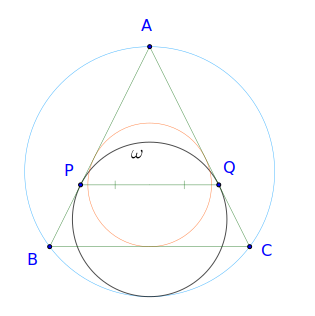
\includegraphics[width=5cm]{./svg/pdf/imo-1978-4-0.pdf}
    \end{center}
\end{frame}

\begin{frame}[t]
    \frametitle{Geometric Transformations}
    \framesubtitle{Homothety - Example 1 - Solution}
    \begin{center}
        \begin{overprint}
            \onslide<1>\centering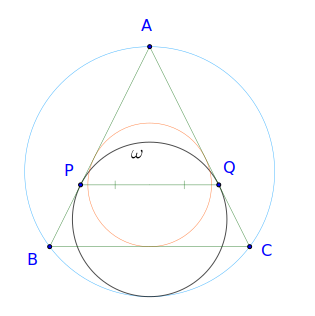
\includegraphics[width=5cm]{./svg/pdf/imo-1978-4-0.pdf}
            \onslide<2->\centering\includegraphics[width=5cm]{./svg/pdf/imo-1978-4-1.pdf}
        \end{overprint}        
    \end{center}
    \begin{overprint}
        \onslide<2>Let $E$ be the center of the circle $\omega$, which is tangent with $AB$, $AC$, and $(ABC)$.
        Let $D$ be the tangent point of the two circles, $M$ be the midpoint of $BC$, and $F$ be the midpoint of $PQ$.
        It is easy to see that $A,F,E,M,D$ are collinear.
        \onslide<3>Let $\mathcal{H}_{(A,k)}$ be a homothety centred at $A$ and $\mathcal{H}_{(A,k)}(D)=M.$
        It is easy to see that $\mathcal{H}_{(A,k)}(E)=F.$
        Let $\gamma$ be the image of $\omega$, $\gamma=\mathcal{H}_{(A,k)}(\omega).$
        Since $\omega$ is tangent $(ABC)$ at $D$, so both are tangent with line $\ell$ through $D$ parallel with $BC,$
        thus $\gamma$ tangent with the image of $\ell$, which is line $BC$.
        \onslide<4>Furthermore, the $\mathcal{H}_{(A,k)}(D)=M,$ keeps $B$ and $C$ on rays $AB$ and $AC$, and because $\omega$ is tangent to $AB$ and $AC$,
        so $\gamma$ is also tangent to $AB$ and $AC$.
        Therefore $\gamma$ is tangent with all sides of $\triangle ABC$, so $\gamma = I_{\triangle ABC}.$
        Therefore, the image of $\mathcal{H}_{(A,k)}(E)$ is $I$, the incentre of $\triangle ABC$, therefore $F \equiv I.$
        Hence, \framebox{the midpoint of $PQ$ is the center of the inscribed circle of the triangle $ABC.$}
    \end{overprint}        
\end{frame}

\end{document}
